\section{Downstream: does the correspondence model matter?}
\label{sec:exp_down}

Correspondence is rarely the end product; it is an input to systems trained around it. Feeding a
pretrained generator a better $IUV$ map at inference proves nothing, because the host is fit to the
error distribution of the correspondence model it was trained with, so a test-time swap measures
distribution shift as much as accuracy. We therefore \emph{retrain the host}, twice; it consumes
only $IUV$, so this tests the correspondence half of our output, not the frame field.
MCLD~\cite{mcld2025} (CVPR'25) is a latent-diffusion~\cite{rombach2022ldm} model that synthesises a
person in a target pose from a source photograph, on DeepFashion In-shop~\cite{liu2016deepfashion},
and it consumes DensePose \emph{twice} --- the source appearance is unwrapped \emph{through} the
source $IUV$ into a $24$-part texture atlas, and the target $IUV$ drives a ControlNet-style pose
guider --- so one upstream change propagates through both branches. Arm~A conditions on detectron2
R101 DensePose~\cite{guler2018densepose,wu2019detectron2} (the authors' released conditions), arm~B
on our model. Fixed across arms: the authors' unmodified code at commit \texttt{6279ff7}, hence their
optimiser, batch size and 60k-step schedule; the original $750\!\times\!1101$ images; seed 12580;
and an \emph{identical} test set ($8{,}512$ pairs). \emph{Both} atlases are regenerated from each
arm's own $IUV$ by the authors' unwrap function, reproducing their released atlases to $0.11\%$
mean absolute difference. Two things are \emph{not} held fixed, so ``one variable'' means ``one
\emph{model}, with what it brings'': arm~B's training list loses $0.07\%$ of arm~A's pairs where
our detector finds no person, and arm~A's conditions carry detectron2's own boxes whereas arm~B
runs our top-down model behind an off-the-shelf detector, so box geometry differs on every image
and the attribution below controls catastrophic failures but not box tightness. Scoring uses the
authors' \texttt{evaluate.py} against their released ground truth, on whose outputs it reproduces
their published numbers to four decimals (LPIPS 0.14817 vs.\ 0.1482, PSNR 18.840 vs.\ 18.84);
arm~A reproduces published MCLD to within 1--2\%. Arm~B is conditioned on \texttt{dp\_w\_F0}@3k
($0.730$ GPS AP), not our headline checkpoint ($0.741$), because the host is trained on the COCO
annotation convention and F0 was the best COCO-convention checkpoint available when the retrains
were launched --- so the result uses the \emph{weaker} of our models. One confound was found and
killed rather than assumed: our first build used the widely mirrored $768\!\times\!1024$
DeepFashion copy, a \emph{per-image} re-crop against which arm~A would have trained mis-aligned to
its own conditions, so we rebuilt on the originals --- and a control arm (arm~A with only its
conditioning warped into mirror geometry) came out \emph{worse} on every paired metric, so that
offset was already learned and never inflated arm~B's margin. MCLD's atlas is also built on the
\textsc{v1} charts, so arm~B inherits the fold ambiguity of \cref{sec:charts} and the measured gain
is a lower bound.

\paragraph{Result.}
Swapping the correspondence model (\cref{tab:mcld}) improves LPIPS~\cite{zhang2018lpips} by
$-0.0117$ ($-7.8\%$) at $256\!\times\!176$ and $-0.0123$ ($-6.9\%$) at $512\!\times\!352$ (where
published MCLD and FPDM score $0.1757$ and $0.1717$),
SSIM~\cite{wang2004ssim} by $+0.0113/{+}0.0080$ and PSNR by $+0.57/{+}0.50$\,dB, with generator,
schedule and data unchanged. Because both arms see the same targets the comparison is paired: the
per-image LPIPS improvement is $+0.0116$, 95\% bootstrap CI $[+0.0110,+0.0123]$, better on $68.7\%$
of images, $d_z=0.371$ at 256, and $+0.0123$, $[+0.0116,+0.0129]$, $72.2\%$, $d_z=0.416$ at 512,
with SSIM and PSNR winning on $72.7\%$/$69.5\%$ and $72.6\%$/$68.9\%$. Wilcoxon gives $p\approx0$
everywhere, which at $n=8{,}512$ says only that the sample is large; the win rates say the gain is
a broad shift of the per-image distribution, not a mean dragged by a few catastrophic failures. But
each arm is \emph{one} training run, so that interval covers image-to-image variability for one
fixed pair of models, not where a second arm-A retrain would land; our only run-level evidence is a
replication across two dataset builds, where the effect measured $-0.0131$ and $-0.0116$ LPIPS
@256, a spread of about $0.0015$, and we quote that spread rather than the interval's lower bound
whenever the comparison is to a quantity of similar size. Nor is the gain merely our model
producing \emph{some} map where detectron2 produces none: detectron2 yields a blank or partial map
on $29$ targets ($0.35\%$) and ours none, but on the $8{,}483$ ($99.66\%$) where \emph{both} maps
are complete the gain is $+0.0114$ at a $68.6\%$ win rate against $+0.0116$/$68.7\%$ overall, so
failures contribute ${\approx}2\%$ of the effect --- robustness (zero detection failures against
detectron2's $29$) being a separate one-line result on studio photography, not a claim about
detection in the wild.

\begin{table}[!tb]
\centering\scriptsize\renewcommand{\arraystretch}{0.94}
\setlength{\tabcolsep}{3.6pt}
\begin{tabular}{lrrrr}
\toprule
Method & FID$\downarrow$ & LPIPS$\downarrow$ & SSIM$\uparrow$ & PSNR$\uparrow$ \\
\midrule
\multicolumn{5}{l}{\emph{$256\times176$}}\\
MCLD~\cite{mcld2025} \emph{(publ.)}      & 6.693 & 0.1482 & 0.7511 & 18.84 \\
FPDM~\cite{fpdm2024} \emph{(publ.)}      & 7.318 & 0.1445 & 0.7417 & 18.832 \\
\cmidrule(lr){1-5}
Arm A ($+$ detectron2 DP)                & \textbf{6.659} & 0.1497 & 0.7462 & 18.656 \\
Arm B ($+$ ours)                         & 6.680 & \textbf{0.1380} & \textbf{0.7575} & \textbf{19.224} \\
$\Delta$ (A$\rightarrow$B)               & \color{gray}$+0.021$ & $-0.0117$ & $+0.0113$ & $+0.568$ \\
\midrule
\multicolumn{5}{l}{\emph{$512\times352$}}\\
Arm A ($+$ detectron2 DP)                & \textbf{6.959} & 0.1781 & 0.7501 & 18.030 \\
Arm B ($+$ ours)                         & 6.963 & \textbf{0.1658} & \textbf{0.7582} & \textbf{18.528} \\
$\Delta$ (A$\rightarrow$B)               & \color{gray}$+0.004$ & $-0.0123$ & $+0.0080$ & $+0.498$ \\
\bottomrule
\end{tabular}
\caption{\textbf{Controlled correspondence swap inside MCLD~\cite{mcld2025}}: two retrains of the
authors' unmodified code differing only in which DensePose produced the conditioning and, through
it, the texture atlas. Every \emph{paired} metric moves and FID~\cite{heusel2017fid} does not
(grey; neutral to marginally \emph{worse}) --- the expected signature for a change that buys
spatial fidelity under a fixed diffusion prior. Published rows come from their authors' harnesses;
FID is not comparable across papers (PIDM~\cite{pidm2023} is 6.36 in MCLD's table, 6.812 in FPDM's)
and we have not verified FPDM's LPIPS is on our axis, so A$\rightarrow$B is the only comparison
here we fully control. One run per arm.}
\label{tab:mcld}
\end{table}

\begin{figure}[!tb]
\centering
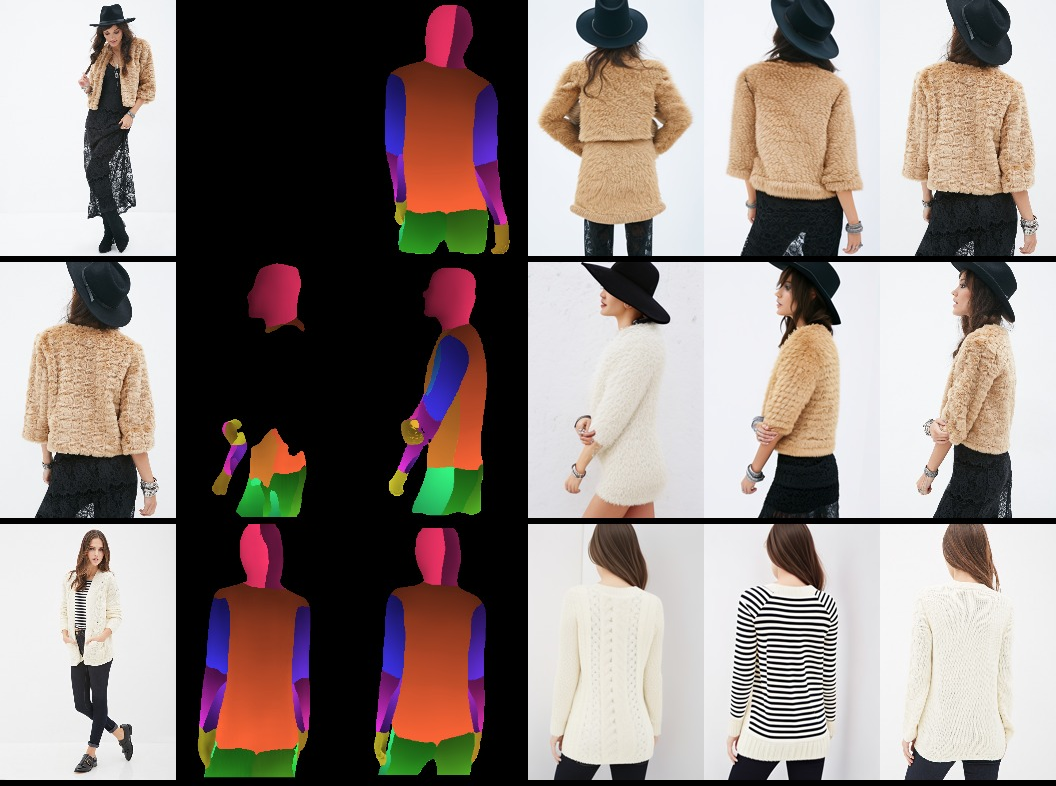
\includegraphics[width=0.86\linewidth]{figs/fig_garment.png}
\caption{\textbf{Garment transfer, rows selected \emph{by} the per-image statistics, not by eye.}
Columns: source; target-pose DensePose from detectron2 and from ours; arm~A; arm~B; ground truth.
Rows: the two largest per-image LPIPS gains and --- for honesty --- the
single worst regression in the test set, where our map drives the generator to unwrap the striped
inner layer instead of the cream knit: the double dependence that produces the gains also
propagates our errors.}
\label{fig:garment}
\end{figure}

\paragraph{Magnitude, and its denominator.}
For scale, the largest published LPIPS step on this benchmark --- our host MCLD to FPDM,
$0.1482\!\rightarrow\!0.1445$ --- is $+0.0037$, and it \emph{cost} SSIM ($-0.0094$) and FID
($+0.63$). Our change is of the same order and does not trade one metric for another, and we stop
there rather than quote a ratio: the numerator is a paired within-host delta from one harness on
identical targets, the denominator a difference between two numbers published by two groups, and
our own reproduction of MCLD differs from its published value by $0.0015$, $40\%$ of that
yardstick. The comparison establishes not a factor but a claim about attention: the correspondence
stage is not a solved input that architecture work can take for granted.

\paragraph{Standing against Leffa, on one axis.}
Leffa~\cite{leffa2025} (CVPR'25) publishes a better LPIPS than ours ($0.114$), but through a
different harness: SqueezeNet LPIPS after a 1024-px resize, against the AlexNet LPIPS of
\cref{tab:mcld}. Rather than argue from published numbers we ran Leffa's released checkpoint
ourselves and scored it and both arms on the \emph{same} $1499$ pairs under \emph{both} harnesses.
Arm~B is ahead of Leffa on every metric on both axes (\cref{tab:leffa}) and closer to
the target on $63.2\%$ of images; so is arm~A, the plain detectron2 baseline. One gap must be stated plainly: our Leffa run does not reproduce Leffa's published
numbers ($0.0969$/$0.687$ against their $0.114$/$0.732$ --- better on LPIPS, worse on SSIM),
plausibly because of our $1499$-pair subset, our generate-then-resize save path, and
pair-construction differences, so we claim a like-for-like comparison on identical inputs, not a
reproduction of their paper. The A$\rightarrow$B delta survives the change of axis
($-0.0070$ @256), so the controlled claim does not depend on which LPIPS is used.

\begin{table}[!tb]\centering\scriptsize\renewcommand{\arraystretch}{0.94}
\setlength{\tabcolsep}{4pt}
\begin{tabular}{@{}lcccccc@{}}
\toprule
 & \multicolumn{3}{c}{VtonEval (squeeze)} & \multicolumn{3}{c}{MCLD (alex)}\\
\cmidrule(lr){2-4}\cmidrule(lr){5-7}
$256$, $n{=}1499$ & LPIPS$\downarrow$ & SSIM$\uparrow$ & PSNR$\uparrow$ & LPIPS$\downarrow$ & SSIM$\uparrow$ & PSNR$\uparrow$\\
\midrule
Leffa (we ran it)  & 0.0969 & 0.6870 & 16.858 & 0.1554 & 0.6845 & 17.452\\
Arm A (detectron2) & 0.0958 & 0.7470 & 17.916 & 0.1494 & 0.7464 & 18.704\\
\textbf{Arm B (ours)} & \textbf{0.0889} & \textbf{0.7580} & \textbf{18.474} & \textbf{0.1379} & \textbf{0.7575} & \textbf{19.299}\\
\bottomrule
\end{tabular}
\caption{Leffa and both MCLD arms on identical pairs under both metric harnesses. Arm~B leads on
every metric on both axes and is closer to the target on $63.2\%$ of images; so does arm~A. Our
Leffa run does \emph{not} reproduce Leffa's published $0.114$/$0.732$ (we measure $0.0969$/$0.687$,
better on LPIPS and worse on SSIM), plausibly because of the $1499$-pair subset, our
generate-then-resize save path and pair construction, so this is a like-for-like comparison on
identical inputs, not a reproduction of their paper.}
\label{tab:leffa}
\end{table}
